\documentclass{article}
\usepackage{maa-monthly}
\usepackage{patrick_custom}
\usepackage{subcaption, tikz-cd}

%% NẾU BẠN ĐÃ CÀI ĐẶT FONT
%\usepackage{mtpro2}
%\usepackage{mathtime}

\graphicspath{{figures/}}

\theoremstyle{theorem}
\newtheorem{theorem}{Định lý}
 
\theoremstyle{definition}
\newtheorem*{definition}{Định nghĩa}
\newtheorem*{remark}{Nhận xét}


\begin{document}

\title{Trực quan hóa các phép quay không gian và các nhóm con hữu hạn của nó}
\markright{Các phép quay và các nhóm con hữu hạn}
\author{}

\maketitle

\begin{abstract}
Bài báo này trình bày cách các nhóm con hữu hạn xuất hiện trong một mô hình tự nhiên của các phép quay không gian phản ánh hình học của một họ các khối đa diện liên quan đến một nhóm quay hữu hạn. Đặc biệt, chúng tôi nhấn mạnh mối quan hệ giữa các lớp liên hợp và các đa diện cụ thể trong không gian quay. 
\end{abstract}


\section{Giới thiệu}
    
    Việc phân loại \emph{các nhóm con hữu hạn của các phép quay không gian}
    \begin{equation}
        \mathrm{FinRot}\coloneqq\curl{G\in \mathrm{Grp}\st G\leq SO(3,\R)\land |G|\in \N}
    \end{equation}
    là đã được biết đến rộng rãi, chúng ta tìm thấy tài liệu tham khảo sớm nhất là Klein vào năm 1888\cite{klein}. Có hai lớp vô hạn: 
    \begin{itemize}
        \item $C_k$ - các nhóm cyclic bậc $k$ là các phép quay của hình chóp $k$-giác
        \item $D_{k}$ - các nhóm dihedral bậc $2k$ là các phép quay của hình lăng trụ $k$-giác
    \end{itemize}
    Đặc biệt, các nhóm $A_4$, $S_4$, và $A_5$ là các nhóm quay của các khối đa diện đều.  Cụ thể: 
    \begin{itemize}
        \item $A_4$ - nhóm xen kẽ trên 4 phần tử, bậc 12, là nhóm đối xứng quay của tứ diện, được biểu diễn như các hoán vị chẵn của các đỉnh. 
        \item $S_4$ - nhóm đối xứng trên 4 phần tử, bậc 24, là các đối xứng quay của hình lập phương, được biểu diễn như các hoán vị của các cặp đỉnh đối diện.
        \item $A_5$ - nhóm xen kẽ trên 5 phần tử, bậc 60, là nhóm đối xứng của hình dodecahedron, bằng hoán vị chẵn của năm cấu trúc tứ diện đồng dạng.
    \end{itemize}  Điều này hoàn thành danh sách các nhóm con hữu hạn của $SO(3)$.
    
    Để trực quan hóa các thành viên của $\mathrm{FinRot}$, trước tiên chúng ta cần một cách trực quan hóa không gian các phép quay; nghĩa là, chúng ta phải có một \emph{không gian thuần nhất chính} cho $SO(3)$ có thể dễ dàng quan sát được. 
    \begin{definition}
       Một \emph{$G$-torsor} hay \emph{không gian thuần nhất chính} cho $G$ là một $G$-Tập \[(T,-\cdot-: G\times T\to T)\] mà hành động của nó là tự do và bắc cầu, tức là: 
       \begin{equation}
           \forall x,y\in T,\exists!  g\in G(y=g\cdot x)
       \end{equation}
    \end{definition}
    Gán cho mỗi điểm $r\coloneqq(x,y,z)^T\in \R^3$ phép quay quanh trục $r$ một góc $|r|$ radian.  Đây được gọi là biểu diễn \emph{trục-góc}. Lưu ý rằng các vectơ cùng hướng với $r$ tương ứng với các phép quay quanh cùng một trục.  Chúng ta biểu diễn các vectơ tương ứng với các ma trận phản đối xứng bởi: 
    \begin{gather}
        r=\begin{bmatrix}
        x \\
        y \\
        z \\
        \end{bmatrix}\mapsto x\hat{x}+y\hat{y}+z\hat{z}=:\hat{r}\\
        \text{ trong đó, }\nonumber\\
        \hat{x} = \begin{bmatrix}
        0 & 0 & 0 \\
        0 & 0 & -1 \\
        0 & 1 & 0
        \end{bmatrix},
        \hat{y} = \begin{bmatrix}
        0 & 0 & 1 \\
        0 & 0 & 0 \\
        -1 & 0 & 0
        \end{bmatrix},
        \hat{z} = \begin{bmatrix}
        0 & -1 & 0 \\
        1 & 0 & 0 \\
        0 & 0 & 0
        \end{bmatrix}
    \end{gather}
    để dấu mũ theo dõi các tính chất đại số của vectơ trừu tượng $r\simeq \hat{r}$ đang được xem xét.  Phép đẳng cấu này cung cấp cho $\R^3$ cấu trúc \emph{đại số Lie} $\so(3)$, với tích Lie: 
    \begin{equation}
        \left[\hat{r}_1,\hat{r}_2\right]\coloneqq\hat{r}_1\hat{r}_2-\hat{r}_2\hat{r}_1
    \end{equation}
    Nó là phản giao hoán và không kết hợp; thỏa mãn:
    \begin{gather}
        \left[\hat{r}_1,\left[\hat{r}_2,\hat{r}_3\right]\right]+\left[\hat{r}_2,\left[\hat{r}_3,\hat{r}_1\right]\right]+\left[\hat{r}_3,\left[\hat{r}_1,\hat{r}_2\right]\right]=0\nonumber\\
        \iff\nonumber\\
        \left[\hat{r}_1,\left[\hat{r}_2,\hat{r}_3\right]\right] = \left[\hat{r}_2,\left[\hat{r}_1,\hat{r}_3\right]\right] +\left[\left[\hat{r}_1,\hat{r}_2\right],\hat{r}_3\right]\label{lder}
    \end{gather}
    Đại số Lie $\so(3)$ là cấu trúc vô cùng nhỏ của $SO(3)$, các vectơ $\hat{r}$ là các đạo hàm hoặc \emph{không gian tiếp xúc} tại phần tử đơn vị với phương trình \ref{lder} định nghĩa quy tắc tích cho các đạo hàm. 
    Bây giờ chúng ta có điều sau đây
    \begin{definition}[Ánh xạ mũ]
       \emph{Ánh xạ mũ} $\exp$ là một ánh xạ trơn từ một \emph{đại số Lie} đến \emph{nhóm Lie} của nó được cho bởi định nghĩa chuỗi lũy thừa tiêu chuẩn trong đại số ma trận trên $\R^3$.  Chúng ta quan tâm đến: 
       \begin{align}
            \exp:\so(3)&\surj SO(3)\\
            \hat{r}&\mapsto \bfr=\sum_{n=0}^\infty\frac{\hat{r}^n}{n!}\nonumber
        \end{align}
        vốn là toàn ánh và gửi $\hat{r}$ đến ma trận $\bfr$ cho phép quay quanh $r$ một góc $|r|$ radian bởi tác động nhân trái thông thường $SO(3)\times \R^3\to \R^3$.
    \end{definition}
    
     Ví dụ $\forall\theta\in\R$: 
    \begin{equation}
        \exp(\theta\hat{x}) = \begin{bmatrix}
        1 & 0 & 0 \\
        0 & \cos{\theta} & -\sin{\theta} \\
        0 & \sin{\theta} & \cos{\theta}
        \end{bmatrix}. 
    \end{equation}
    là một phép quay quanh $(1,0,0)^T$ một góc $\theta$ radian.
    
    Ánh xạ này là toàn ánh trong trường hợp này vì $SO(3)$ là compact và liên thông \cite[Cor. 11.10]{hall}, tức là \emph{mọi} phép quay được biểu diễn dưới dạng $\exp(\hat{r})$ cho một số $\hat{r}\in\so(3)$.
    Lưu ý các phép quay tầm thường (đơn vị) bởi $2\pi$ theo bất kỳ hướng nào đều tương đương với không làm gì cả: 
    \begin{equation}
        (\hat{0} \sim \hat{r})\iff \hat{r} \in 2\pi\Z S^2\subseteq \so(3)
    \end{equation}
    trong đó $S^2:=\{s\in \R^3\st |s| = 1\}$ là mặt cầu đơn vị. 
    
    Nếu không, các phép quay không tầm thường quanh cùng một trục mà khác nhau một bội số nguyên của $2\pi$ là giống nhau, điều này định nghĩa quan hệ tương đương: 
    \begin{equation}
       \forall \hat{r}_1, \hat{r}_2\in\so(3)\setminus2\pi\Z S^2 \left((\hat{r}_1\sim \hat{r}_2)\iff\land
       \begin{cases}
       \exists s\in \R&\st\hat{r}_1=s\hat{r}_2\\
       \exists t\in 2\pi\Z&\st|r_1-r_2|=t
       \end{cases}
       \right)
    \end{equation}
    
    Điều này tạo ra \emph{ánh xạ thương}
    \begin{align}
        q:  \so(3)&\surj \so(3)/\sim \\
        \hat{r} &\mapsto [\hat{r}] \coloneqq \curl{\hat{r}'\in\so(3)\st \hat{r}'\sim \hat{r}}
    \end{align}
    là toàn ánh lên tập hợp các lớp tương đương được gọi là \emph{không gian thương} khi được trang bị \emph{tô pô thương}:  $\Top{q}$.  Bây giờ chúng ta có thể quan sát rằng biểu diễn trục-góc phân tích thành một cách tự nhiên, thông qua ánh xạ mũ: 
    \begin{equation}
        \begin{tikzcd}
        \so(3) \arrow[d, two heads, "q"'] \arrow[rd, two heads, "\exp"] & \\
        \so(3)/\sim \arrow[r, dashed, hook, two heads, "!", "\eta"'] & SO(3)
        \end{tikzcd}
    \end{equation}
    Trên thực tế $\eta$ là một \emph{phép đồng phôi}: 
    \begin{itemize}
        \item \emph{đơn ánh}\begin{align*}
            \forall&[\hat{x}_1],[\hat{x}_2]\in\so(3)/\sim\\
            [\hat{x}_1]\neq [\hat{x}_2]&\implies \exp(\hat{x}_1)\neq \exp(\hat{x}_2)\\
            &\implies \eta([\hat{x}_1])\neq\eta([\hat{x}_2])
        \end{align*}
        \item \emph{toàn ánh}\begin{align*}
            \forall \mathbf{X}\in SO(3), \exists \hat{x}\in\so(3)\st \exp(\hat{x})=\mathbf{X}\\
            \implies \exists [\hat{x}]\in\so(3)/\sim\st \eta([\hat{x}])=\mathbf{X}
        \end{align*}
        \item \emph{mở}---$\forall U\in\tau_{q}, \eta(U) = \exp(q^{-1}(U))\in \Top{SO(3)}$, điều này đúng vì $q$ liên tục theo tính chất của ánh xạ thương và, trong trường hợp này, $\exp$ là ánh xạ mở\cite[Thm. 3.31]{hall}.
    \end{itemize}
    Chúng ta nói rằng $\exp$ \emph{phân tích} thành $\eta\circ q$.  Bởi vì $\eta$ là một phép đồng phôi, ánh xạ thương $q$ là hình thái tô pô của $\exp$; nó nắm bắt cơ chế thay đổi từ toàn ánh sang song ánh. 
    
    Việc dán $q$ là vấn đề trung tâm của trực quan hóa đối với chúng ta. Một việc dán như vậy là không thể thực hiện về mặt cơ học trong chỉ ba chiều, chúng ta sẽ cần một chiều thứ tư để uốn cong vào để cho phép một thao tác như vậy. Thay vào đó, chúng ta nghiên cứu một nghịch đảo trái $p$ của $q$ bằng cách xác định nó một cách rõ ràng trên một miền trong $\so(3)$ phục vụ như một $SO(3)$-torsor.
    
    Chúng ta định nghĩa $p$ là ảnh ngược của $q$ cắt với một tập con của $\so(3)$ sao cho $p$ được định nghĩa tốt. Xét quả cầu mở bán kính $\pi$ trong $\so(3)$:
    \begin{equation}
        B\coloneqq\curl{\hat{r}\in\so(3)\st |r|<\pi}
    \end{equation}
    
    $B$ là \emph{gần như} một $SO(3)$-torsor; nó có các đại diện duy nhất cho tất cả các phép quay ngoại trừ các phép quay chính xác $\pi$. Để sửa $B$ chúng ta cho nó một ``mũ'' $\hem$ của các phép quay $\pi$ duy nhất.  Định nghĩa
    \begin{equation}
        \hem\coloneqq\curl{\hat{r}\in\partial B\st z>0\lor (z=0\land y>0)\lor x=\pi}
    \end{equation}
    lưu ý rằng tập hợp hơi tùy tiện này có các tính chất quan trọng sau:
    \begin{gather}
        \hat{r}=\pi\frac{\hat{r}}{|r|}\in \hem\implies -\hat{r}=-\pi\frac{\hat{r}}{|r|}\not\in \hem\label{pnp}\\
        \partial B=\hem\sqcup -\hem\label{djb}
    \end{gather}
    Một khi định nghĩa
    \begin{equation}
        \overline{B}\coloneqq B\sqcup \hem,
    \end{equation}
    hàm $p$ là một nghịch đảo phải của $q$ gửi mỗi lớp tương đương $[\hat{r}]$ đến phần tử duy nhất của $[\hat{r}]\cap\overline{B}$. Theo cách này các phép quay $\pi$ được gán cho các đại diện duy nhất, ngăn việc chọn cả $\hat{r}$ và $-\hat{r}$ (tại các cực đối diện trên $\partial B$):
    \begin{align}
        p:\so(3)/\sim &\inj \so(3) \\
        [\hat{x}]&\overset{! }{\mapsto} \hat{x}'\in [\hat{x}]\cap\overline{B}
    \end{align}
    sao cho $p$ chọn một đại diện duy nhất cho mỗi lớp tương đương trong $\so(3)/\sim$. Lưu ý ảnh bằng $\overline{B}$, được hiển thị trong Hình \ref{fig:log-so3}.  \emph{Mọi hình trong bài báo này là một hình chiếu của $\overline{B}$ lên một mặt phẳng. } Mỗi lớp tương đương $[\hat{r}]\in\so(3)/\sim$ trong sơ đồ giao hoán: 
    \begin{equation}\label{pimcd}
        \begin{tikzcd}
        \exp^*(\curl{\bfr})\arrow[r, hook] \arrow[d] & \so(3)\arrow[d, "\exp"] \\
        \curl{\bfr}\arrow[r, hook] & SO(3)
        \end{tikzcd}
    \end{equation}
    \begin{figure}
        \centering
        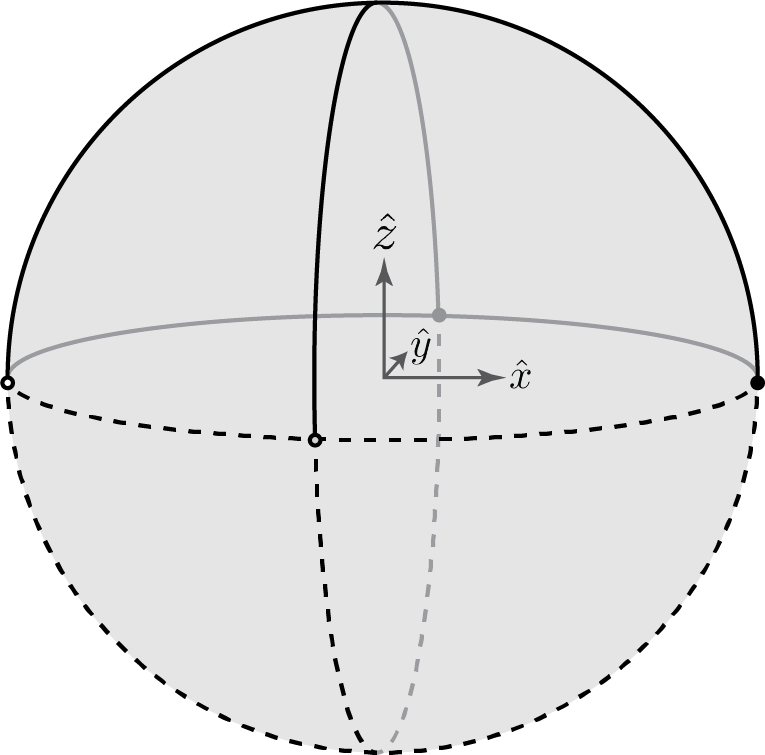
\includegraphics{log-so3-diagram}
        \caption{
        Sơ đồ của $\overline{B}$. Các đường liền và đứt chỉ ra $\overline{B}$ có và không chứa biên của nó.
        }
        \label{fig:log-so3}
    \end{figure}
    luôn cắt $\overline{B}$ đúng một lần. 
    \begin{definition}[Ảnh ngược và Ảnh]
       \emph{Ảnh ngược} $f^*$ của một hàm $f: A\to B$ là một hàm giữa các tập lũy thừa $f^*:\pow{B}\to\pow{A}$, thỏa mãn sơ đồ giao hoán như trong phương trình \ref{pimcd}, tức là:
       \begin{equation}\label{def: pim}
           f^*(S)\coloneqq\curl{x\in A\st f(x)\in S\subseteq B}
       \end{equation}
       Theo ký hiệu này, \emph{ảnh} $f_*$ là: 
       \begin{equation}\label{def:im}
           f_*(S)\coloneqq\curl{f(x)\in B\st x\in S\subseteq A}
       \end{equation}
       sao cho $f_*:\pow{A}\to\pow{B}$.  Khi có một phần tử đơn vị $\id\in B$, \emph{nhân} $\ker f\coloneqq f^*(\id)$ là ảnh ngược của nó.
    \end{definition}
    Vì các phép quay $2\pi$ là phần tử đơn vị, chúng ta có $\ker\exp\coloneqq\exp^*{\id}=2\pi\Z S^2\subset \so(3)$.
    Cho $\bfr\neq \id\in SO(3)$ và một số $\hat{r}\in\exp^*(\bfr)$, thì phải có trường hợp
    \begin{equation}
        \exp^*(\bfr)=\hat{r}+2\pi \Z\frac{\hat{r}}{|r|}\subset \mathfrak{so}(3)
    \end{equation}
    một lần nữa vì các phép quay $2\pi$ là phần tử đơn vị; các vectơ đồng tuyến trong đại số Lie khác nhau về độ lớn bởi một bội số nguyên của $2\pi$ phải ánh xạ đến cùng một giá trị dưới ánh xạ mũ. 
    
    Một lần nữa cho m���t số $\bfr\neq\id \in SO(3)$, chỉ một $z\in \Z$ cho một điểm trong quả cầu nửa đóng, $\overline{B}$, vì đường kính của nó là $2\pi$ và nó chứa nhiều nhất một trong bất kỳ cặp cực đối diện nào. Đây là định nghĩa của ánh xạ logarit:
    \begin{align}
        \log: SO(3)&\inj \so(3) \\
        \bfr&\mapsto \hat{r}\in\exp^*(\bfr)\cap \overline{B} = p\circ \eta^{-1}(\bfr)
    \end{align}
    %Do đó $B/\sim$ là một \emph{không gian thuần nhất chính} cho $SO(3)$. (không thực sự sử dụng định nghĩa của PHS, có lẽ thay đổi điều này) Tôi đặt tên phần tử duy nhất $\log(\bfr)\coloneqq\exp^{-1}(\bfr)\cap\overline{B}$ là nghịch đảo logarit.
    Mọi sơ đồ mô tả $\log_*(G)\subset\overline{B}=\log_*(SO(3))\subset\so(3)$ trong đó $G\in \mathrm{FinRot}$, tức là mọi trực quan hóa là một cái nhìn \emph{cắt} của $SO(3)$, bởi vì $\log$ là nghịch đảo trái của $\exp$ trên $\overline{B}$: 
    \begin{equation}
        \begin{tikzcd}
           & SO(3)\arrow[dr, hook, "\log"] & \\
           \so(3) \arrow[ur, two heads, "\exp"]\arrow[rr, "\id"]&& \so(3)
        \end{tikzcd}
    \end{equation}
    Chúng ta tập trung vào $\overline{B}$ vì nó là một $SO(3)$-torsor dưới tác động (kiểm tra điều này!)
    \begin{align}
        SO(3)\times \so(3)&\to \so(3)\\
        (\G,\hat{x})&\mapsto \log(\G\exp{\hat{x}})\nonumber
    \end{align}
    
    Trước đó chúng ta gọi ảnh của $G$ dưới $\log$ là ``làm phẳng'' của nhóm con đó. Chúng ta chọn tên này như một phép ẩn dụ dựa trên cách ánh xạ mũ hoạt động đối với các số thuần ảo:  một song ánh từ đường thẳng ảo đến đường tròn đơn vị, cũng là giá trị tuyệt đối của số phức trong các số phức đơn vị.
    
    Đối với các nhóm con hữu hạn, việc đặt các đại diện phần tử nhóm trong các bản vẽ của chúng ta bị giới hạn bởi bậc: 
    \begin{theorem}\label{thm:sphereclass}
        Nếu một phần tử $\G\in G\leq SO(3)$ có bậc $\left|\G\right|=n\in\N$, thì đại diện của nó $\hat{g}=\log(\G)\in \overline{B}$ phải nằm trong một mặt cầu bán kính $|g|=2\pi k/n$ trong đó 
        \begin{equation*}
            (2k\leq n)\land (k|n\implies k=1).
        \end{equation*}
    \end{theorem}
    \begin{proof}
    Theo giả thiết: 
    \begin{equation}
        \id = \G^n = \exp(n\hat{g})
    \end{equation}
    Quan hệ tương đương $\sim$, tức là các phép quay bởi $2\pi$ là phần tử đơn vị, hàm ý có một $k\in\Z$ trong đó
    \begin{equation}
        n\hat{g}=2\pi k\frac{\hat{g}}{|g|}\implies |g|=\frac{2\pi k}{n}
    \end{equation}
    trong khi $\hat{g}\in \overline{B}$ nên $2\pi k/n\leq \pi$ do đó $2k\leq n$. Giả sử $k|n$, thì
    \begin{gather}
        \exp(\hat{g}n/k)=\exp(2\pi \hat{g}/|g|)=\id\\
        \implies\G^{n/k}=\G^n=\id
    \end{gather} và $n$ là số nguyên nhỏ nhất trong đó $\G^n=\id$, do đó $k = 1$.
    \end{proof}
    Hơn nữa, với mọi $k\in \N$ thỏa mãn điều trên, có một phần tử
        \begin{equation*}
            \G^k=\exp\left(\frac{k}{n}\frac{2\pi \hat{g}}{\left|g\right|}\right)\in G
        \end{equation*}
    cũng có bậc $n$, như có thể thấy bởi điều kiện không chia hết $k|n\implies k=1$. 
    Định lý này giới hạn việc đặt các đại diện trong $\overline{B}$ vào các mặt cầu đồng tâm tại gốc tọa độ với bán kính $2\pi k/n$ cho các đối xứng bậc $n$. Điều này cùng với tính đối xứng quay cho biết các phần tử trong một lớp liên hợp phải nằm trên cùng một mặt cầu. 
    
\section{Các khối đa diện dẫn xuất}

Chúng tôi làm theo cảm hứng từ Hatcher \cite{MR1867354} trong ký hiệu, định nghĩa một điểm hoặc \emph{0-ô}, và định nghĩa đệ quy đĩa mở đơn vị $n$ chiều hoặc \emph{$n$-ô} là
\begin{gather}
    e^0\coloneqq \star\\
    e^n\coloneqq \curl{(x,y)\in \R\times e^{n-1}\subseteq \R^n\st x^2+||y||^2<1}
\end{gather}
sao cho chỉ số trên theo dõi chiều ô. 
Coi như cho trước một khối đa diện $P$ được thực hiện như một phức CW 2 chiều hữu hạn ô phẳng nhúng trong $\R^3$ và đồng phôi với mặt cầu, được trang bị nhóm lớn nhất $\rot{P} \coloneqq G\leq SO(3)$ tác động tự do lên $P$, qua: 
\begin{align}
    \alpha: G\times P&\to P\\
    (\G,x)&\mapsto \G\cdot x\nonumber
\end{align}
\begin{definition}[Tính đều đặn]
    Chúng ta gọi $n=|\rot{P}|$ là \emph{tính đều đặn} của khối đa diện $P$. Do đó các khối đa diện với tác động nhóm tự do lớn là \emph{đều đặn}.
\end{definition}
\begin{definition}[Các ô liền kề và vỏ]
    Một cặp ô $e^i_a, e^j_b\in P$ là liền kề $e^i_a ||| e^j_b$ nếu một trong hai là một phần của biên của cái kia. 
    \begin{equation}
        e^i_a ||| e^j_b \defeq e^i_a \subset \partial e^j_b || e^j_b\subset\partial e^i_a
    \end{equation}
    Tập hợp các ô liền kề với một ô cho trước là vỏ của nó.
    \begin{equation}
        \shell{e^i_a}\coloneqq \{e^j_b\in P\st e^i_a|||e^j_b\}
    \end{equation}
\end{definition}
Như một phức CW, $P$ là một hợp rời rạc $P^0\sqcup P^1\sqcup P^2$, được gọi là một \emph{phân ô}, của nó: 
\begin{itemize}
    \item các đỉnh được đặt tên $P^0$ (0-ô). Chính thức là một họ hữu hạn $J$ chỉ số của các ánh xạ từ singleton $P^0\coloneqq\curl{e^0_j: e^0\to \R^3}_{j\in J}$ với tất cả các ảnh khác biệt $(i\neq j\implies e^0_i\neq e^0_j)$.
    \item các cạnh được đặt tên $P^1$ (1-ô). Một họ các ánh xạ liên tục $P^1\coloneqq\curl{e^1_{ij}:  e^1\to \R^3}_{(i,j)\in K}$ được chỉ số bởi một tập con $K\subseteq J\times J=J^2$ sao cho $(i,j)\in K$ ngụ ý cặp $\curl{e^0_i, e^0_j}$ có khoảng cách tối thiểu giữa các đỉnh: 
    \begin{equation}
        |e^0_i-e^0_j|=\min \curl{|e^0_{i'}-e^0_{j'}|}_{(i',j')\in J^2}
    \end{equation}
    Chúng ta sử dụng các đoạn, được định nghĩa là hàm của $t\in e^1$, thỏa mãn: 
    \begin{equation}
        e^1_{ij}(t)\coloneqq\frac{(t+1)e^0_j-(t-1)e^0_i}{2}
    \end{equation}
    sao cho $\partial e^1_{ij}=\curl{e^0_i, e^0_j}$; chúng là các đoạn phẳng (thẳng) treo giữa các cặp 0-ô liền kề.
     
    Một 1-ô tổng quát có thể vòng từ một đỉnh về chính nó, tuy nhiên đối với một khối đa diện được định nghĩa theo cách này mọi cạnh kết thúc ở hai điểm khác biệt, biên $\partial e^1_{ij}$. 
    \item  các mặt được đặt tên $P^2$ (2-ô). Một họ các ánh xạ liên tục $P^2\coloneqq\curl{e^2_{\Delta}:  e^2\to \R^3}$ được chỉ số bởi các vòng cạnh $\Delta$, sao cho $\partial e^2_{\Delta}=\Delta$.  
\end{itemize}

Một vòng đồng phẳng (có thể không phân biệt) có thể được gán cho mỗi 1-phức con có dạng
\begin{gather*}
    e^1_{ijk}\coloneqq\curl{e^0_i,e^1_{ij}, e^0_j, e^1_{jk}, e^0_k}\\
    \st \paren{\sum_{\ell\in \curl{i,j,k}}\lambda_\ell e^0_\ell = 0\implies \lambda_\ell = 0}
\end{gather*}
một đường đi với 3 đỉnh độc lập tuyến tính nhưng liền kề $e^0_j$, như $\Delta\coloneqq\partial\paren{P\cap e^2_{ijk}}=e^1_{jk\dots ij}:  S^1\simeq\partial e^2\hookrightarrow \R^3$ trong đó $e^2_{ijk}$ là ảnh của bao lồi co của 3 điểm trong $\R^3$. 
Theo cách này khối đa diện có một số tính chất đại số đẹp: 
\begin{gather}
    \partial P^d = \bigsqcup_{c<d}P^c\label{pbd}\\
    G\cdot P^d\coloneqq\curl{g\cdot x\in P\st (g,x)\in G\times P^d}=P^d\label{cinv}\\
    \sum_{d=0}^2(-1)^d|P^d|=2\label{eucha}
\end{gather}
 Tính chất \ref{pbd} là theo định nghĩa để xây dựng một phức ô hữu hạn.  Tính chất \ref{cinv} phát biểu rằng nhóm phải ổn định độc lập mỗi loại ô. Cuối cùng tính chất \ref{eucha} là đặc số Euler của các khối đa diện đồng phôi với mặt cầu.
%  Điều này ngay lập tức cho một tập hợp các đồng cấu liên kết cho mọi $i\in\curl{0,1,2}$: 
%  \begin{gather}
%      \phi_{i}: G\to S_{|P^i|}
%  \end{gather}
%  bằng cách theo dõi tác động nhóm trên $P^i$ riêng biệt. 

 Có một số khối đa diện bất biến dưới cùng một tác động nhóm được tạo ra bằng cách thay thế các $d$-ô liên quan bằng các 0-ô trọng tâm của chúng, sau đó tạo ra một khối đa diện mới từ các đỉnh này như trước đây. Một ví dụ quen thuộc là khối đối ngẫu. 
 
 \begin{definition}[Các ô tương tự]
    Chúng ta nói một cặp ô $A, B\subseteq P^n$ là \emph{tương tự} nếu tồn tại một $\G\in G$ sao cho $A=\G\cdot B\coloneqq\curl{\G\cdot b\st b\in B}$ như các tập hợp. 
 \end{definition}
 \begin{theorem}[Các ô tương tự có vỏ tương tự]
     Nếu $A, B\subseteq P^n$ là các ô tương tự, thì các vỏ $\shell{A}, \shell{B}$ của mỗi cái phải được cấu thành từ các ô tương tự tương ứng 1-1.  Điều này là do tác động $\G$ hoạt động trên toàn bộ khối đa diện: 
     \begin{gather}
         \G\cdot A= B\implies \G\cdot \partial A = \partial B\\
         \G\cdot \shell{A} = \{\G\cdot A'|||\G\cdot A = B|A'|||A\} = \shell{B}
     \end{gather}
    
 \end{theorem}
 Đối với các khối đa diện: 
 Vỏ của một 0-ô luôn là ``cánh hoa'' xen kẽ của các 2-ô và biên 1-ô của chúng.  Vỏ của một 1-ô luôn là một cặp mỗi loại gồm 0-ô (biên của 1-ô) và 2-ô (các mặt có 1-ô là một phần của biên). Vỏ của một 2-ô luôn là một vòng 1-ô và các 0-ô liền kề với chúng. 

 Hầu hết các đối xứng khối đa diện đều đặn là bắc cầu trên các đỉnh nên tất cả các 0-ô đều tương tự. Tuy nhiên hầu hết các kim cương dihedral có một cặp điểm đối diện không tương tự với phần lớn các điểm chu vi khác.
 
 Nói chung không phải tất cả các 2-ô $P^2$ của $P$ đều tương tự, tức là chúng không có cùng hình dạng tô pô theo nghĩa bao nhiêu 0-ô và 1-ô tạo thành biên của nó. Nếu một cặp 2-ô $A,B$ không tương tự thì chúng có thể có các vỏ không tương tự.
 Tuy nhiên $P$ là đều đặn nếu và chỉ nếu mọi 2-ô đều tương tự (kiểm tra điều này).
 \begin{definition}[Khối đa diện dẫn xuất]
    Một \emph{khối đa diện dẫn xuất} được tạo ra bằng cách đặt một đỉnh tại trọng tâm của mỗi phức con đơn tương tự của $P$, sau đó tạo ra một khối đa diện mới một cách đệ quy từ các đỉnh này như trước
 \end{definition}
 
 Xét tập hợp tất cả các phức con
 \begin{equation}\label{def:subc}
     \subc{P}\coloneqq\curl{C\subseteq P: C\text{ là một phức ô đóng}}
 \end{equation}
Chúng ta có thể phân hoạch tập hợp các phức con 
\begin{equation}
    \subc{P}=\bigsqcup_{s\in S}\Orb_s
\end{equation}
 theo tính tương tự $S$, như các quỹ đạo $\Orb_s\coloneqq G\cdot C_s$ của \emph{đẩy tiến} của $\alpha$: 
 \begin{align}
     \alpha_*: G\times\subc{P}&\to \subc{P}\\
     (\G, C)&\mapsto \G\cdot C\nonumber\\
     \text{trong đó, } G\cdot C\coloneqq \curl{\G\cdot x\in P\st(\G, x)\in G\times C}\nonumber
 \end{align}
 Là tác động được cảm sinh bởi tất cả các phép nhúng của các phức con $C$ vào $P$. Chúng ta diễn giải các quỹ đạo này như các lớp tương tự của các hình dạng, trong đó bởi hình dạng chúng ta có nghĩa là một sắp xếp cụ thể của các ô trong không gian. 
 
 Đặc biệt quan tâm đối với chúng ta là các lớp tương tự hoặc lớp \emph{hình dạng} $\Orb^d_s\coloneqq G\cdot C^d_s\in \subc{P^d}/G$ của các phức $d$-ô đơn khác nhau $C^d_s\coloneqq e^d_s\sqcup \partial e^d_s$. 
 Tuy nhiên $d=2$ là trường hợp đầu tiên mà một $d$-ô đơn có thể không tương tự với cái khác. Cụ thể: 
 \begin{itemize}
     \item $d=0$, thì biên $\partial e^0_j$ là rỗng, và mỗi cặp 0-ô đơn với vỏ tương tự đều tương tự.
     \item $d=1$, thì biên $\partial e^1_{ij}$ là cặp $\curl{e^0_i, e^0_j}$ và vì vậy mỗi 1-ô đơn trong một khối đa diện tương tự với một phức con đồng phôi với khoảng đóng $[0,1]$. 
     \item $d=2\implies \partial e^2_n=\Delta_n$ trong đó $\Delta_n=e^1_{jk\dots ij}$ và $jk\dots ij$ có độ dài $n$ và chỉ định một phức con 1-vòng với $n$ cạnh treo tuần tự giữa $n$ đỉnh.  Trong trường hợp này một $e^2_n$ tương tự với một $n$-gon.
 \end{itemize}
 
%  Cho một $d$-ô $S\in P^d$, gán $S$ \emph{bộ ổn định} $G_S$ của nó, nhóm con của $G$ cố định $S$, và lưu ý rằng các phức con tương tự có các bộ ổn định liên hợp và ngược lại. 
%  \begin{align*}
%      A=g\cdot B\iff G_A &= G_{g\cdot B}\\
%      &=\curl{h\in G: g\cdot B = hg\cdot B}\\
%      &=\curl{h\in G:  B = g^{-1}hg\cdot B}\\
%      &=\curl{h\in G: g^{-1}hg\in G_B}\\
%      &=gG_Bg^{-1}
%  \end{align*}
 
Chúng ta phân tích phân hoạch thành $\bigsqcup_{s\in S}\Orb^d_s$ bằng cách xét tác động của \emph{bộ ổn định} $G^d_s$ của một số $C^d_s$ trên phức con biên của nó, trong đó trường hợp không tầm thường đầu tiên là $d=2$: 
\begin{align}
    \partial C^2_s=\bigsqcup_{e^0_j\in \partial C^d_s}e^0_j\sqcup\bigsqcup_{e^1_{ij}\subseteq\partial C^d_s}e^1_{ij}
\end{align}
\emph{Định lý quỹ đạo-bộ ổn định} cho chúng ta biết rằng: 
\begin{equation}
    |\Orb^d_i|=\left[G: G^d_i\right]
\end{equation}
sao cho đặc biệt số lượng các ô con tương tự trong $P$ phải chia hết bậc của $G$. 
 
Một khối đa diện dẫn xuất $D_i P^d$ tồn tại cho mỗi quỹ đạo $\Orb^d_i$ trong $\subc{P^d}/G$ mà các đỉnh $|\Orb^d_i|$ của nó được cho bởi các trọng tâm của các $i$-ô trong $\Orb^d_i$. 
 
Khối đối ngẫu của một khối đa diện đều đặn ở trên là một loại khối đa diện dẫn xuất.  Bởi vì mọi 1-ô của $P$ đều tương tự, vì mỗi cái là một khoảng mở bị giới hạn bởi một cặp đỉnh khác biệt do đó ổn định bởi nhóm tầm thường, khối đối ngẫu là khối đa diện dẫn xuất từ $\Orb^2_0$.
 
Một câu hỏi thú vị cho nghiên cứu tiếp theo là:  quá trình này tổng quát hóa như thế nào đến các chiều cao hơn?
 
\section{Các nhóm cyclic và dihedral}

\begin{figure}
    \centering
    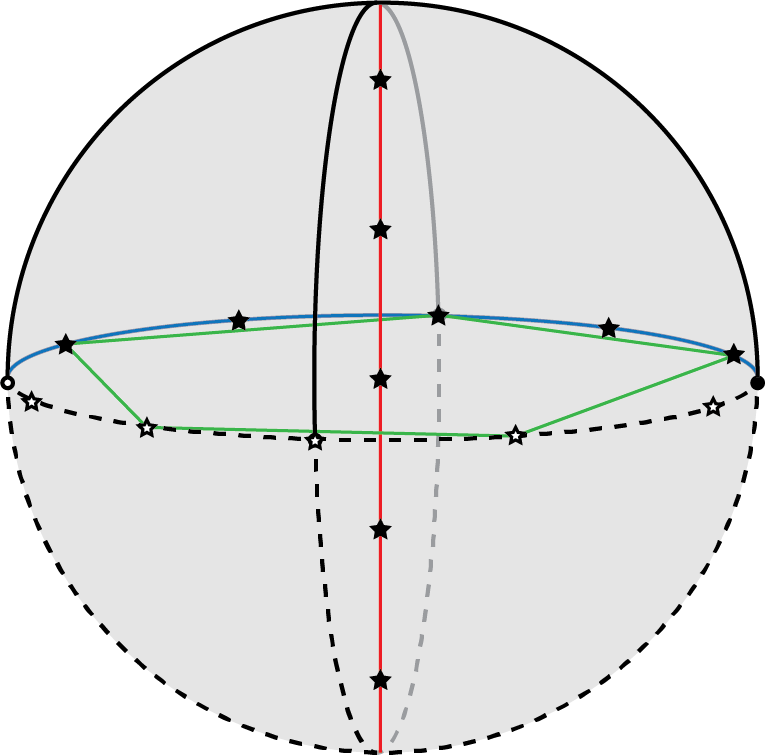
\includegraphics{d5-in-so3}
    \caption{$D_5\leq SO(3,\R)$ được minh họa trong $\overline{B}$}
    \label{fig: D5inSO3}
    \caption{Các ngôi sao không tô màu là cùng một điểm với các ngôi sao tô màu đối diện trên vòng tròn ngũ giác xanh dưới đồng nhất thức chênh lệch $2\pi$}
\end{figure}

$C_k$ là một nhóm con của $D_k$, vì vậy chúng ta sẽ giới hạn trực quan hóa của mình với nhóm sau; nhóm trước chỉ là một tập con của sơ đồ.  Xét $D_5$, các đối xứng của ngũ giác đều.  Không mất tính tổng quát chúng ta căn chỉnh ngũ giác trong $\R^3$ sao cho các phép quay về một đỉnh là quanh trục $z$ và một cạnh nằm song song với mặt phẳng $xy$. 

Trong sơ đồ này (Hình \ref{fig:D5inSO3}), các ngôi sao là các phần tử nhóm.  Nhóm con $C_5$ của các phép quay quanh trục $z$ là các ngôi sao dọc theo đường đỏ thẳng đứng. Đồng đẳng của nhóm con đó, các phép lật, nằm trên vòng tròn xanh.  Các ngôi sao không tô màu trên biên là các vị trí tương đương với các ngôi sao tô màu ở cực đối diện dưới đồng nhất thức $2\pi$.

Trên thực tế có một ngũ giác khác trong hình này, mặc dù nó bị che khuất bởi việc làm phẳng $SO(3)$ của chúng ta, năm ngôi sao trên đường đỏ, chứa các \emph{5-chu trình}. Vì $n=5$, $k=1,2$ là các giá trị duy nhất thỏa mãn điều kiện trong Định lý \ref{thm:sphereclass}, do đó có hai ngũ giác đan xen bán kính $2\pi/5$ và $4\pi/5$ lồng nhau.

Đường xanh và đường đỏ là một cặp \emph{vòng tròn lớn} lồng nhau, và các ngôi sao cách đều trên các vòng tròn này, \emph{làm cho $D_5$ là một cặp ngũ giác đều lồng nhau nhúng trong $SO(3)$}.

Tôi chỉ trình bày một ví dụ này và để người đọc xem xét các nhóm dihedral khác (và các nhóm con cyclic) sẽ xuất hiện như thế nào trong sơ đồ này.  Điều gì thay đổi khi nhóm dihedral trên một ngũ giác lẻ hoặc một ngũ giác chẵn? 
\section{Các nhóm xen kẽ và đối xứng}
$A_4$ là một nhóm con của $S_4$ nên một lần nữa chúng ta chuyển sang thảo luận về nhóm sau.  Đây là các đối xứng quay của cả hai đối tượng đối ngẫu là lục diện (hình lập phương) và bát diện, cũng như một khối Archimedean, khối lập phương bát diện.

\begin{figure}[h]
    \begin{subfigure}{. 49\linewidth}
    \centering
    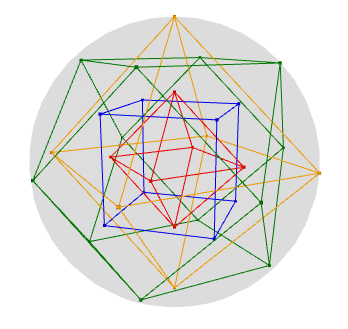
\includegraphics[width = \linewidth]{s4}
    \caption{$S_4$ được minh họa trong $\overline{B}$}
    \end{subfigure}
    \begin{subfigure}{.49\linewidth}
    \centering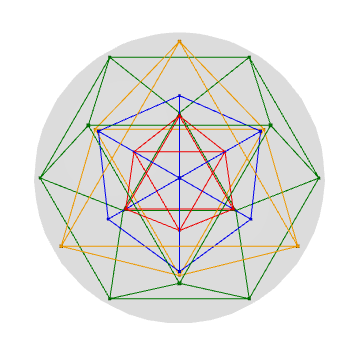
\includegraphics[width=\linewidth]{s4-3cycle}
    \caption{nhìn dọc theo trục 3-chu trình}
    \end{subfigure}
    \begin{subfigure}{.49\linewidth}
    \centering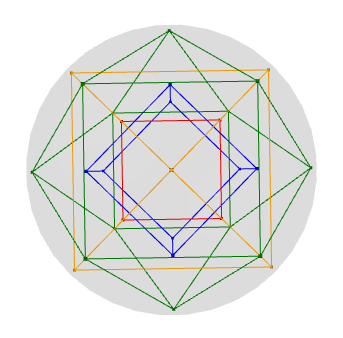
\includegraphics[width=\linewidth]{s4-4cycle}
    \caption{nhìn dọc theo trục 4-chu trình}
    \end{subfigure}
    \begin{subfigure}{.49\linewidth}
    \centering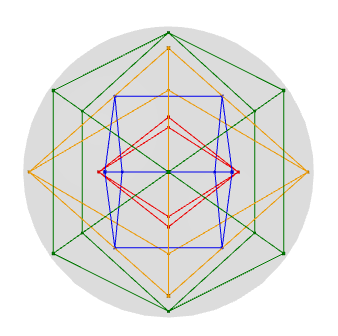
\includegraphics[width=\linewidth]{s4-2cycle}
    \caption{nhìn theo trục 2-chu trình}
    \end{subfigure}
    \caption{
        Các lớp liên hợp là các khối đa diện mã màu \\\centering
        \begin{tabular}{c|c}
            bát diện đỏ & 4-chu trình \\
            hình lập phương xanh & 3-chu trình \\
            bát diện vàng & 2-2-chu trình \\
            khối lập phương bát diện xanh lá & 2-chu trình
        \end{tabular}
    }
    \label{fig:s4}
\end{figure}

Xét các 3-chu trình trong $S_4$ khi nó tác động lên hình lập phương.  Mỗi trong 8 phần tử này phải cố định một trong các đường chéo của hình lập phương, chúng là một phép quay quanh trục đó. 3-chu trình có bậc 3, vì vậy các đại diện của chúng phải nằm trong một mặt cầu bán kính $2\pi/3$. Do đó chúng tạo thành một hình lập phương bán kính $2\pi/3\approx 2.09$, vừa khít trong $\overline{B}$.

Còn 4-chu trình thì sao? đây là các phép quay quanh các trục đi qua tâm của các mặt đối diện của hình lập phương, hoặc tương đương, cố định các trục qua các đỉnh đối diện trong bát diện đối ngẫu. Có 6 trong số đó, bậc 4, và như vậy tạo thành một bát diện bán kính $2\pi/4=\pi/2\approx 1.57$. 

3 2-2-chu trình là bình phương của 4-chu trình, và do đó có cùng trục quay. \emph{Chúng cũng là một bát diện}, nhưng bây giờ bán kính $\pi$ nên các cực đối diện của nó được đồng nhất như yêu cầu bởi $\sim$:  chúng nằm trên $\partial B$.

Cuối cùng, 6 2-chu trình cố định các đường chéo qua các trung điểm đối diện của các cạnh hình lập phương.  Khối đa diện được tạo thành bởi các điểm này là một khối lập phương bát diện. Các đại diện phải n���m trong một mặt cầu bán kính $\pi$ nên chúng cũng nằm trên $\partial\overline{B}$.

\begin{figure}[h]
    \begin{subfigure}{.49\linewidth}
    \centering
    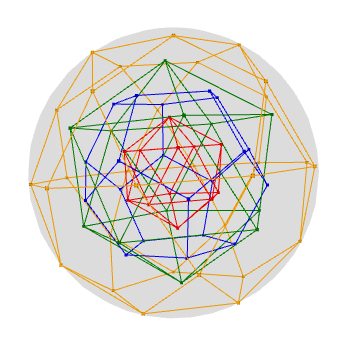
\includegraphics[width=\linewidth]{a5}
    \caption{$A_5$ được minh họa trong $\overline{B}$}
    \end{subfigure}
    \begin{subfigure}{.49\linewidth}
    \centering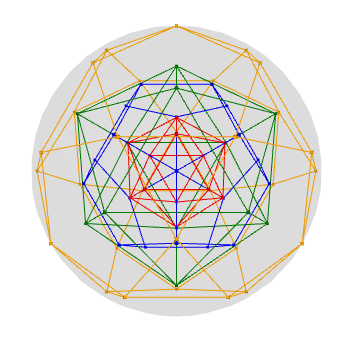
\includegraphics[width=\linewidth]{a5-3cycle}
    \caption{nhìn dọc theo trục 3-chu trình}
    \end{subfigure}
    \begin{subfigure}{.49\linewidth}
    \centering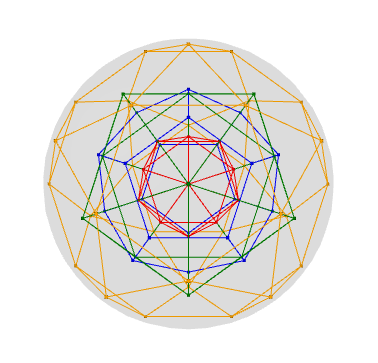
\includegraphics[width=\linewidth]{a5-5cycle}
    \caption{nhìn dọc theo trục 5-chu trình}
    \end{subfigure}
    \begin{subfigure}{.49\linewidth}
    \centering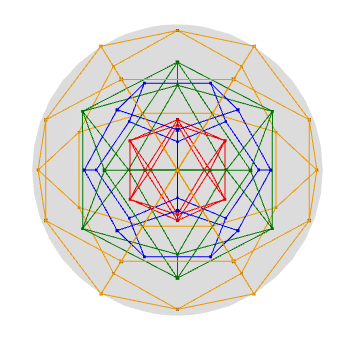
\includegraphics[width=\linewidth]{a5-2-2cycle}
    \caption{nhìn dọc theo trục 2-2-chu trình}
    \end{subfigure}
    \caption{
        Các lớp liên hợp là các khối đa diện mã màu \\\centering
        \begin{tabular}{c|c}
            icosahedron đỏ & 5-chu trình ($k=1$) \\
            dodecahedron xanh & 3-chu trình \\
            icosahedron xanh lá & 5-chu trình ($k=2$) \\
            icosidodecahedron vàng & 2-2-chu trình
        \end{tabular}
    }
    \label{fig:a5}
\end{figure}

Lưu ý rằng $A_4 = S_4^2=<(123), (12)(34)>\subset S_4$ chỉ là các 3-chu trình và các 2-2-chu trình vì: 
\begin{itemize}
    \item 2-chu trình và 2-2-chu trình bình phương thành phần tử đơn vị
    \item 3-chu trình được gửi đến 3-chu trình, và 4-chu trình đến 2-2-chu trình bởi phép bình phương
\end{itemize}
Tương đương, các đối xứng của một tứ diện là một hình lập phương và một nửa bát diện, hoặc một loại ``tam giác'' đều; một đối tượng hình học với 3 đỉnh được nối bằng các cạnh có độ dài bằng nhau nhúng trong không gian.

Quá trình này hoạt động gần như chính xác cùng một cách đối với $A_5$ (hình \ref{fig:a5}) như các đối xứng của dodecahedron với một sự khác biệt quan trọng do 5-chu trình tách thành hai lớp liên hợp. 
\begin{itemize}
    \item 3-chu trình cố định các đỉnh của một dodecahedron và có bậc 3, vì vậy các đại diện của chúng là một dodecahedron bán kính $2\pi/3$. 
    \item 5-chu trình cố định các đỉnh của icosahedron đối ngẫu và có bậc 5, vì vậy các đại diện của chúng là một \emph{cặp} icosahedra đối ngẫu, một b��n kính $2\pi/5$ và một $4\pi/5$.
    \item 2-2-chu trình cố định các đỉnh của icosidodecahedron đối ngẫu trung điểm cạnh\footnote{của cả dodecahedron và icosahedron} và có bậc 2, vì vậy các đại diện của chúng là các cặp đỉnh đối diện trên $\partial B$.
\end{itemize}

\section{Kết luận}
Hình học của chính các nhóm hữu hạn có liên quan mật thiết đến hình học của các đối tượng m
